\documentclass{beamer}
%https://en.wikibooks.org/wiki/LaTeX/Macros
\usepackage{tikz}
%vectors, matrices, complex numbers, big O notation, grafentheorie, vertaling van probleem in algoritme, trigonometrie

\newcommand{\drawtdvec}[2]{
\draw[step=1cm,gray,very thin] (-3,-3) grid (3,3);
\draw[red, thick, ->] (0,0) -- (#1,#2);
\draw[thick,->] (0,0) -- (3,0) node[anchor=north west] {x};
\draw[thick,->] (0,0) -- (0,3) node[anchor=south east] {y};
\end{tikzpicture}
}

\newcommand{\drawbasicvec}{
		\begin{equation*} \vec{V} = \begin{bmatrix} 1 \\ 2 \end{bmatrix} \end{equation*}
				\begin{tikzpicture}[scale=0.70]
        \drawtdvec{1}{2}
}


\title{Some math}
\subtitle{Random things you might encounter in the core or afterwards}

%\usetheme{lucid}
\begin{document}
	\frame {
		\titlepage
	}
	\frame {
		\frametitle{Vector}
%draw arrow
\begin{columns}
\begin{column}{0.5\textwidth}
		\drawbasicvec
\end{column}

\begin{column}{0.5\textwidth}
%draw arrow, in 6 dimensions
		\begin{equation*} \textbf{U} = \begin{bmatrix} 0.2 \\ 0.5 \\ 0.7 \\ 0.2 \\ 0.2 \\ 0.2 \end{bmatrix} \end{equation*}
				\begin{tikzpicture}[scale=0.70]
\draw[step=1cm,gray,very thin] (-3,-3) grid (3,3);
\draw[red, thick, ->] (0,0) -- (1.1,1.7);
\draw[thick,->] (0,0) -- (3,0);
\draw[thick,->] (0,0) -- (0,3);
\end{tikzpicture}
\end{column}
\end{columns}
	}
	\frame {
		\frametitle{Scaling a vector}
%draw arrow
\begin{columns}
\begin{column}{0.5\textwidth}
		\drawbasicvec
\end{column}

\begin{column}{0.5\textwidth}
%draw arrow, in 6 dimensions
		\begin{equation*} 1.5 * \vec{V} = \begin{bmatrix} 1.5 \\ 3  \end{bmatrix} \end{equation*}
				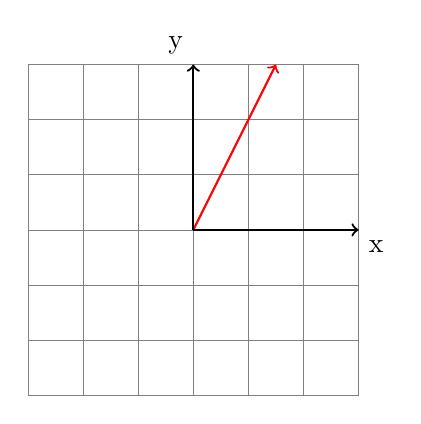
\begin{tikzpicture}[scale=0.70]
\draw[step=1cm,gray,very thin] (-3,-3) grid (3,3);
\draw[red, thick, ->] (0,0) -- (1.5,3);
\draw[thick,->] (0,0) -- (3,0) node[anchor=north west] {x};
\draw[thick,->] (0,0) -- (0,3) node[anchor=south east] {y};
\end{tikzpicture}
\end{column}
\end{columns}


	}
	\frame {
		\frametitle{Scaling with negative number}
		\drawbasicvec
		\begin{equation*} \textbf{U} = \begin{bmatrix} 0.2 & 0.3 \\ 0.5 & 0.6 \end{bmatrix} \end{equation*}
	}
	\frame {
		\frametitle{Matrix}
		\begin{equation*} \textbf{U} = \begin{bmatrix} 0.2 & 0.3 \\ 0.5 & 0.6 \end{bmatrix} \end{equation*}
	}
	\frame {
		\frametitle{ABC formula}
		\[\frac{-b \pm \sqrt{b^2 - 4 a c}}{2a}\]
	}
	\frame{
		\frametitle{Sample Page 2}
		\framesubtitle{An Example of Lists}
		\begin{itemize}
			\item 1
			\item 2
			\item 3
		\end{itemize}
	}
	\frame{
	    \frametitle{Paragraph Content}
	    This is a paragraph.
	}
\end{document}
